\chapter{Experimentos e Resultados} \label{cap:Resultados}

Este capítulo apresenta os resultados obtidos através da execução experimental do algoritmo de balanceamento de carga proposto, comparando-o com as estratégias convencionais de \textit{Round-Robin} e Seleção Aleatória. Os experimentos foram conduzidos nos quatro cenários definidos no Capítulo~\ref{cap:Proposta}, variando a carga do sistema (100 e 1000 usuários simultâneos) e a configuração dos servidores (homogênea e heterogênea).

A análise desses dados permite avaliar objetivamente a eficácia do algoritmo proposto em diferentes condições de operação e validar as hipóteses estabelecidas no Capítulo \ref{cap:Proposta}.

\section{Cenários de Teste}

A avaliação experimental do algoritmo proposto foi conduzida através de múltiplos cenários de teste, projetados para avaliar o desempenho do sistema sob diferentes condições de carga e configurações de recursos dos servidores. Os cenários foram cuidadosamente definidos para permitir uma análise comparativa rigorosa entre as diferentes estratégias de balanceamento de carga.

\subsection{Parâmetros Globais}

Todos os cenários de teste compartilham os seguintes parâmetros:

\begin{itemize}
    \item \textbf{\textit{Timeout} de requisição}: 30 segundos
    \item \textbf{Número de vídeos no catálogo}: 12
    \item \textbf{Número de resoluções disponíveis}: 6 (conforme descrito na seção anterior)
\end{itemize}

\subsection{Definição dos Cenários}

Foram definidos quatro cenários principais, cada um testado com três estratégias de balanceamento diferentes (\textit{Round-Robin}, Seleção Aleatória e Monitoramento de Memória com diferentes intervalos de atualização). A Tabela \ref{tab:test-scenarios} apresenta a especificação detalhada de cada cenário.

\begin{table}[htbp]
\centering
\caption{Cenários de teste definidos para avaliação experimental}
\label{tab:test-scenarios}
\small
\begin{tabular}{|c|c|c|p{6.5cm}|}
\hline
\textbf{Cenário} & \textbf{Usuários} & \textbf{Distribuição} & \textbf{Configuração dos Servidores} \\
\hline
1 & 100 & Heterogênea & 
\textbf{S1}: 4096MB / 1024MB/s; \newline
\textbf{S2}: 2048MB / 512MB/s; \newline
\textbf{S3}: 1024MB / 256MB/s; \newline
\textbf{S4}: 512MB / 128MB/s; \newline
\textbf{S5}: 256MB / 64MB/s; \newline
\textbf{S6}: 128MB / 32MB/s; \newline
\textbf{S7}: 64MB / 16MB/s; \newline
\textbf{S8}: 32MB / 8MB/s \\
\hline
2 & 100 & Homogênea & 
Todos os servidores: 1024MB RAM e 256MB/s de leitura \\
\hline
3 & 1000 & Heterogênea & 
Mesma configuração do Cenário 1 \\
\hline
4 & 1000 & Homogênea & 
Mesma configuração do Cenário 2 \\
\hline
\end{tabular}
\end{table}

\subsection{Descrição dos Cenários}

\subsubsection{Cenário 1: Baixa Concorrência com Servidores Heterogêneos}

Este cenário simula uma situação de carga moderada com 100 usuários simultâneos acessando um conjunto de servidores com capacidades significativamente diferentes. A heterogeneidade dos recursos visa avaliar a capacidade do algoritmo proposto de identificar e priorizar servidores com maior disponibilidade de recursos. Espera-se que estratégias que ignoram o estado dos servidores (como \textit{Round-Robin} e Seleção Aleatória) distribuam a carga de forma uniforme, potencialmente sobrecarregando os servidores menos capazes, enquanto o algoritmo de monitoramento de memória deve ser capaz de direcionar mais requisições para os servidores com maior capacidade.

\subsubsection{Cenário 2: Baixa Concorrência com Servidores Homogêneos}

Este cenário mantém o mesmo nível de carga do Cenário 1, mas utiliza servidores com recursos idênticos. O objetivo é avaliar o comportamento das estratégias em um ambiente onde não há vantagem teórica em favorecer um servidor específico. Neste cenário, espera-se que todas as estratégias apresentem desempenho similar, uma vez que a distribuição uniforme de carga é adequada quando os servidores possuem capacidades equivalentes.

\subsubsection{Cenário 3: Alta Concorrência com Servidores Heterogêneos}

Este cenário eleva significativamente a carga do sistema para 1000 usuários simultâneos, mantendo a configuração heterogênea de servidores. O objetivo é avaliar o comportamento das estratégias sob condições de alta pressão, onde a capacidade de identificar e evitar servidores sobrecarregados torna-se crítica para manter a qualidade de serviço. Este é o cenário mais exigente e onde se espera observar as maiores diferenças de desempenho entre as estratégias.

\subsubsection{Cenário 4: Alta Concorrência com Servidores Homogêneos}

O último cenário combina alta carga com servidores homogêneos, oferecendo um ponto de comparação para o Cenário 3. Ele permite avaliar se as diferenças observadas no Cenário 3 são devidas à heterogeneidade dos recursos ou ao nível de carga do sistema.

\subsection{Estratégias de Balanceamento Avaliadas}

Para cada um dos quatro cenários descritos, foram executados testes com as seguintes estratégias de balanceamento:

\begin{enumerate}
    \item \textbf{\textit{Round-Robin}}: Estratégia de linha de base que distribui as requisições de forma cíclica entre os servidores.
    
    \item \textbf{Seleção Aleatória}: Estratégia de linha de base que seleciona um servidor aleatoriamente para cada requisição.
    
    \item \textbf{Monitoramento de Memória (intervalo médio de 6 segundos)}: Algoritmo proposto com intervalo médio de atualização de métricas de 6 segundos, representando um cenário com informações relativamente atualizadas.
    
    \item \textbf{Monitoramento de Memória (intervalo médio de 30 segundos)}: Algoritmo proposto com intervalo médio de atualização de 30 segundos, representando um cenário com informações moderadamente desatualizadas.
\end{enumerate}

Cada combinação de cenário e estratégia de balanceamento foi implementada como uma \textit{branch} Git específica no repositório do projeto, permitindo o isolamento e a reprodutibilidade de cada configuração experimental. Esta organização através de \textit{branches} facilitou a execução sistemática dos testes e garantiu que as diferentes configurações não interferissem entre si.

A avaliação com diferentes intervalos de atualização visa demonstrar a robustez do algoritmo proposto mesmo quando operando com informações de carga moderadamente obsoletas, uma situação comum em sistemas distribuídos de larga escala onde o custo de monitoramento muito frequente pode ser proibitivo.

\section{Análise comparativa}

A validação da eficácia do algoritmo proposto foi realizada por meio de uma análise comparativa rigorosa, executada em cenários de baixa e alta carga. Para estabelecer uma condição de teste relevante, o sistema foi submetido a uma carga de trabalho constante, gerada pelo \textit{script} cliente que realiza múltiplas requisições paralelas.

A metodologia de avaliação será centrada em métricas quantitativas que impactam tanto direta quanto indiretamente a QoE do usuário final. Durante a execução de cada cenário de teste - que consiste na reprodução de uma sessão de um vídeo do começo ao fim - As métricas coletadas são as seguintes: O número total de travamentos (\textit{stalls}) do vídeo, o \textit{bitrate}, a \textbf{qualidade média} de reprodução ao longo da sessão e a latência média de obtenção de cada segmento na sessão completa. Essas métricas oferecem uma visão objetiva do desempenho de cada estratégia de balanceamento, tanto sob estresse quanto sob condições normais de uso.

O algoritmo proposto, baseado na interpretação de sobrecarga de servidores mediante ao monitoramento de memória, será comparado com duas abordagens clássicas e amplamente utilizadas: \textit{Round-Robin} e Seleção Aleatória. Para assegurar uma comparação justa, a mesma aplicação de balanceamento de carga desenvolvida em Rust será utilizada em todos os testes, alterando-se apenas o módulo de decisão do algoritmo. Serão executados os seguintes cenários:

\begin{enumerate}
    \item{Balanceamento com algoritmo \textit{Round-Robin}.}
    \item{Balanceamento com algoritmo de Seleção Aleatória.}
    \item{Balanceamento com o algoritmo proposto, utilizando um intervalo médio de atualização dos dados dos servidores de 6 segundos.}
    \item{Balanceamento com o algoritmo proposto, utilizando um intervalo médio de atualização dos dados dos servidores de 30 segundos.}
\end{enumerate}

A escolha de 6 e 30 segundos para os intervalos médios dos dois cenários do balanceamento com o algoritmo proposto foi realizada apenas para gerar resultados comparativos entre dois intervalos significativamente diferentes. A hipótese central é que o algoritmo proposto, mesmo com informações moderadamente desatualizadas (no intervalo de 30s), apresentará um desempenho superior em termos de QoE quando comparado aos métodos \textit{Round-Robin} e Aleatório. Adicionalmente, espera-se que, entre as variações do algoritmo proposto, o intervalo de 6 segundos forneça os melhores resultados, enquanto o intervalo de 30 segundos demonstrará a capacidade do algoritmo de manter bom desempenho mesmo com dados menos atualizados.

\section{Visão Geral dos Resultados}

A Tabela \ref{tab:latency-results} apresenta a latência média de resposta observada em cada combinação de cenário e estratégia de balanceamento. A latência representa o tempo médio necessário para que uma requisição HTTP seja completada, sendo um indicador direto da eficiência do balanceamento de carga e da utilização dos recursos do sistema.

\begin{table}[htbp]
\centering
\begin{threeparttable}
\caption{Latência média de resposta (em milissegundos) por cenário e estratégia de balanceamento}
\label{tab:latency-results}
\small
\begin{tabular}{|l|c|c|c|c|}
\hline
\textbf{Estratégia} & \textbf{Cenário 1} & \textbf{Cenário 2} & \textbf{Cenário 3} & \textbf{Cenário 4} \\
\hline
Round-Robin & 2345,5 & 78,6 & 3988,4 & 610,6 \\
\hline
Seleção Aleatória & 2163,3 & 72,2 & 2878,1 & 610,6 \\
\hline
MM (6s) & \textbf{336,6} & \textbf{71,4} & \textbf{1197,2} & \textbf{619,6} \\
\hline
MM (30s) & 604,6 & 73,1 & 2183,3 & 671,3 \\
\hline
\end{tabular}

\begin{tablenotes}
\footnotesize
%\item[*] Significant differences compared to the model using all scores (All).
\item MM = Monitoramento de Memória.
\end{tablenotes}

\end{threeparttable}
\end{table}

%\noindent\small{MM = Monitoramento de Memória}

Os resultados de latência revelam padrões importantes. Nos cenários com servidores heterogêneos (Cenários 1 e 3), o algoritmo de monitoramento de memória com intervalo de 6 segundos apresentou reduções dramáticas de latência: 85,7\% no Cenário 1 e 70,0\% no Cenário 3 em comparação com \textit{Round-Robin}. Nos cenários homogêneos (Cenários 2 e 4), todas as estratégias apresentaram latências similares, indicando que a heterogeneidade dos recursos é um fator determinante para a eficácia do balanceamento inteligente.

A Tabela \ref{tab:stalls-results} resume os eventos de travamento observados em cada configuração. Travamentos representam pausas forçadas na reprodução do vídeo devido à falta de dados no \textit{buffer} do cliente, sendo um dos principais fatores de degradação da QoE.

\begin{table}[htbp]
\centering
\caption{Resumo de travamentos por cenário e estratégia}
\label{tab:stalls-results}
\small
\begin{tabular}{|l|c|c|c|c|}
\hline
\textbf{Estratégia} & \textbf{Qtd.} & \textbf{Duração (s)} & \textbf{Cenário} & \textbf{Maior (s)} \\
\hline
\multicolumn{5}{|c|}{\textbf{Cenário 1: 100 usuários, heterogêneo}} \\
\hline
Round-Robin & 1 & 6,62 & 1 & 6,62 \\
Seleção Aleatória & 0 & 0,00 & 1 & -- \\
MM (6s) & 0 & 0,00 & 1 & -- \\
MM (30s) & 0 & 0,00 & 1 & -- \\
\hline
\multicolumn{5}{|c|}{\textbf{Cenário 2: 100 usuários, homogêneo}} \\
\hline
\multicolumn{5}{|c|}{Nenhum travamento observado em qualquer estratégia} \\
\hline
\multicolumn{5}{|c|}{\textbf{Cenário 3: 1000 usuários, heterogêneo}} \\
\hline
Round-Robin & 7 & 15,12 & 3 & 8,16 \\
Seleção Aleatória & 8 & 29,72 & 3 & 13,38 \\
MM (6s) & 0 & 0,00 & 3 & -- \\
MM (30s) & 4 & 6,42 & 3 & 3,83 \\
\hline
\multicolumn{5}{|c|}{\textbf{Cenário 4: 1000 usuários, homogêneo}} \\
\hline
\multicolumn{5}{|c|}{Nenhum travamento observado em qualquer estratégia} \\
\hline
\end{tabular}
\end{table}

Os dados de travamentos evidenciam a superioridade do algoritmo de monitoramento de memória, especialmente no Cenário 3 (alta concorrência com servidores heterogêneos), onde as estratégias convencionais falharam completamente. O algoritmo com intervalo de 6 segundos eliminou totalmente os travamentos nos cenários críticos, enquanto o intervalo de 30 segundos apresentou apenas 4 travamentos de curta duração, demonstrando robustez mesmo com dados moderadamente obsoletos.

\section{Métricas}

Conforme descrito no Capítulo \ref{cap:Implementacao}, durante cada execução experimental foram coletadas métricas detalhadas de QoE ao longo de toda a sessão de reprodução de vídeo. Os dados brutos --- sequências de qualidades escolhidas pelo \textit{player}, \textit{bitrate} estimado por segmento, eventos de \textit{stalling} e latências médias --- foram exportados em formato JSON e posteriormente processados pelos scripts localizados na pasta \texttt{src/chart-generators}, que geraram os gráficos consolidados armazenados em \texttt{./Textuais/5-ExperimentosEResultados/outputs}. Esta seção apresenta e discute essas métricas, comparando sistematicamente os quatro cenários e as quatro estratégias de balanceamento avaliadas.

\subsection{Qualidade}

A qualidade de reprodução foi monitorada como a sequência de resoluções MPEG-DASH selecionadas pelo cliente ao longo dos segmentos de vídeo, mapeadas em uma escala ordinal de 1 a 6, correspondente a 144p, 240p, 360p, 480p, 720p e 1080p, respectivamente. As Figuras~\ref{fig:quality-scenario-1} a~\ref{fig:quality-scenario-4} apresentam a evolução da qualidade ao longo do tempo para cada cenário de teste, comparando as estratégias \textit{Round-Robin}, Seleção Aleatória e Monitoramento de Memória com intervalos médios de atualização de 6 e 30 segundos.

\begin{figure}[htbp]
    \centering
    
\includegraphics[width=0.75\linewidth]{./Textuais/5-ExperimentosEResultados/outputs/quality-charts/scenario-1.png}
    \caption{Evolução da qualidade de vídeo no Cenário 1 (100 usuários, servidores heterogêneos).}
    \text{Fonte: Elaborado pelo autor (2025).}
    \label{fig:quality-scenario-1}
\end{figure}

\begin{figure}[htbp]
    \centering
    
\includegraphics[width=0.75\linewidth]{./Textuais/5-ExperimentosEResultados/outputs/quality-charts/scenario-2.png}
    \caption{Evolução da qualidade de vídeo no Cenário 2 (100 usuários, servidores homogêneos).}
    \text{Fonte: Elaborado pelo autor (2025).}
    \label{fig:quality-scenario-2}
\end{figure}

\begin{figure}[htbp]
    \centering
    
\includegraphics[width=0.75\linewidth]{./Textuais/5-ExperimentosEResultados/outputs/quality-charts/scenario-3.png}
    \caption{Evolução da qualidade de vídeo no Cenário 3 (1000 usuários, servidores heterogêneos).}
    \text{Fonte: Elaborado pelo autor (2025).}
    \label{fig:quality-scenario-3}
\end{figure}

\begin{figure}[htbp]
    \centering
    
\includegraphics[width=0.75\linewidth]{./Textuais/5-ExperimentosEResultados/outputs/quality-charts/scenario-4.png}
    \caption{Evolução da qualidade de vídeo no Cenário 4 (1000 usuários, servidores homogêneos).}
    \text{Fonte: Elaborado pelo autor (2025).}
    \label{fig:quality-scenario-4}
\end{figure}

Nos cenários com servidores heterogêneos (Cenários 1 e 3), observa-se um contraste marcante entre as estratégias baseadas em estado (\textit{Monitoramento de Memória}) e as estratégias que ignoram a carga dos servidores. No Cenário 1, \textit{Round-Robin} e Seleção Aleatória exibem quedas abruptas e prolongadas para resoluções baixas (sobretudo 144p e 240p), refletindo períodos em que parte dos usuários é direcionada a servidores mais limitados. Em contrapartida, as variantes de Monitoramento de Memória mantêm a maior parte da sessão em 1080p, com oscilações pontuais e curtas para resoluções intermediárias, indicando melhor utilização dos servidores mais capazes.

No Cenário 3, sob alta concorrência e heterogeneidade, o padrão se intensifica: as estratégias \textit{Round-Robin} e Aleatória degradam rapidamente a qualidade para níveis mínimos (predominância de 144p e 240p), enquanto o algoritmo proposto com intervalos de 6s e 30s consegue sustentar resoluções altas (720p e 1080p) durante praticamente toda a sessão. Isso evidencia que o monitoramento de recursos consegue evitar a concentração de requisições em servidores já saturados, preservando a qualidade mesmo em condições adversas.

Nos cenários homogêneos (Cenários 2 e 4), as curvas de qualidade das quatro estratégias são muito próximas: em geral, todas mantêm a reprodução em 1080p, com poucas oscilações. Nesses ambientes, como esperado, a distribuição uniforme de requisições é naturalmente adequada, e o ganho proporcionado pelo algoritmo proposto em termos de qualidade percebida é pequeno, ainda que ele mantenha desempenho comparável sem prejuízo à QoE.

\subsection{Bitrate}

O \textit{bitrate} por segmento representa a taxa de transferência medida pelo \textit{player} MPEG-DASH para cada requisição de segmento, em \si{\kilo\bit\per\second}. Esta métrica quantifica a capacidade efetiva da infraestrutura em fornecer dados ao cliente ao longo do tempo. As Figuras~\ref{fig:bitrate-scenario-1} a~\ref{fig:bitrate-scenario-4} apresentam a evolução do \textit{bitrate} por cenário e estratégia de balanceamento.

\begin{figure}[htbp]
    \centering
    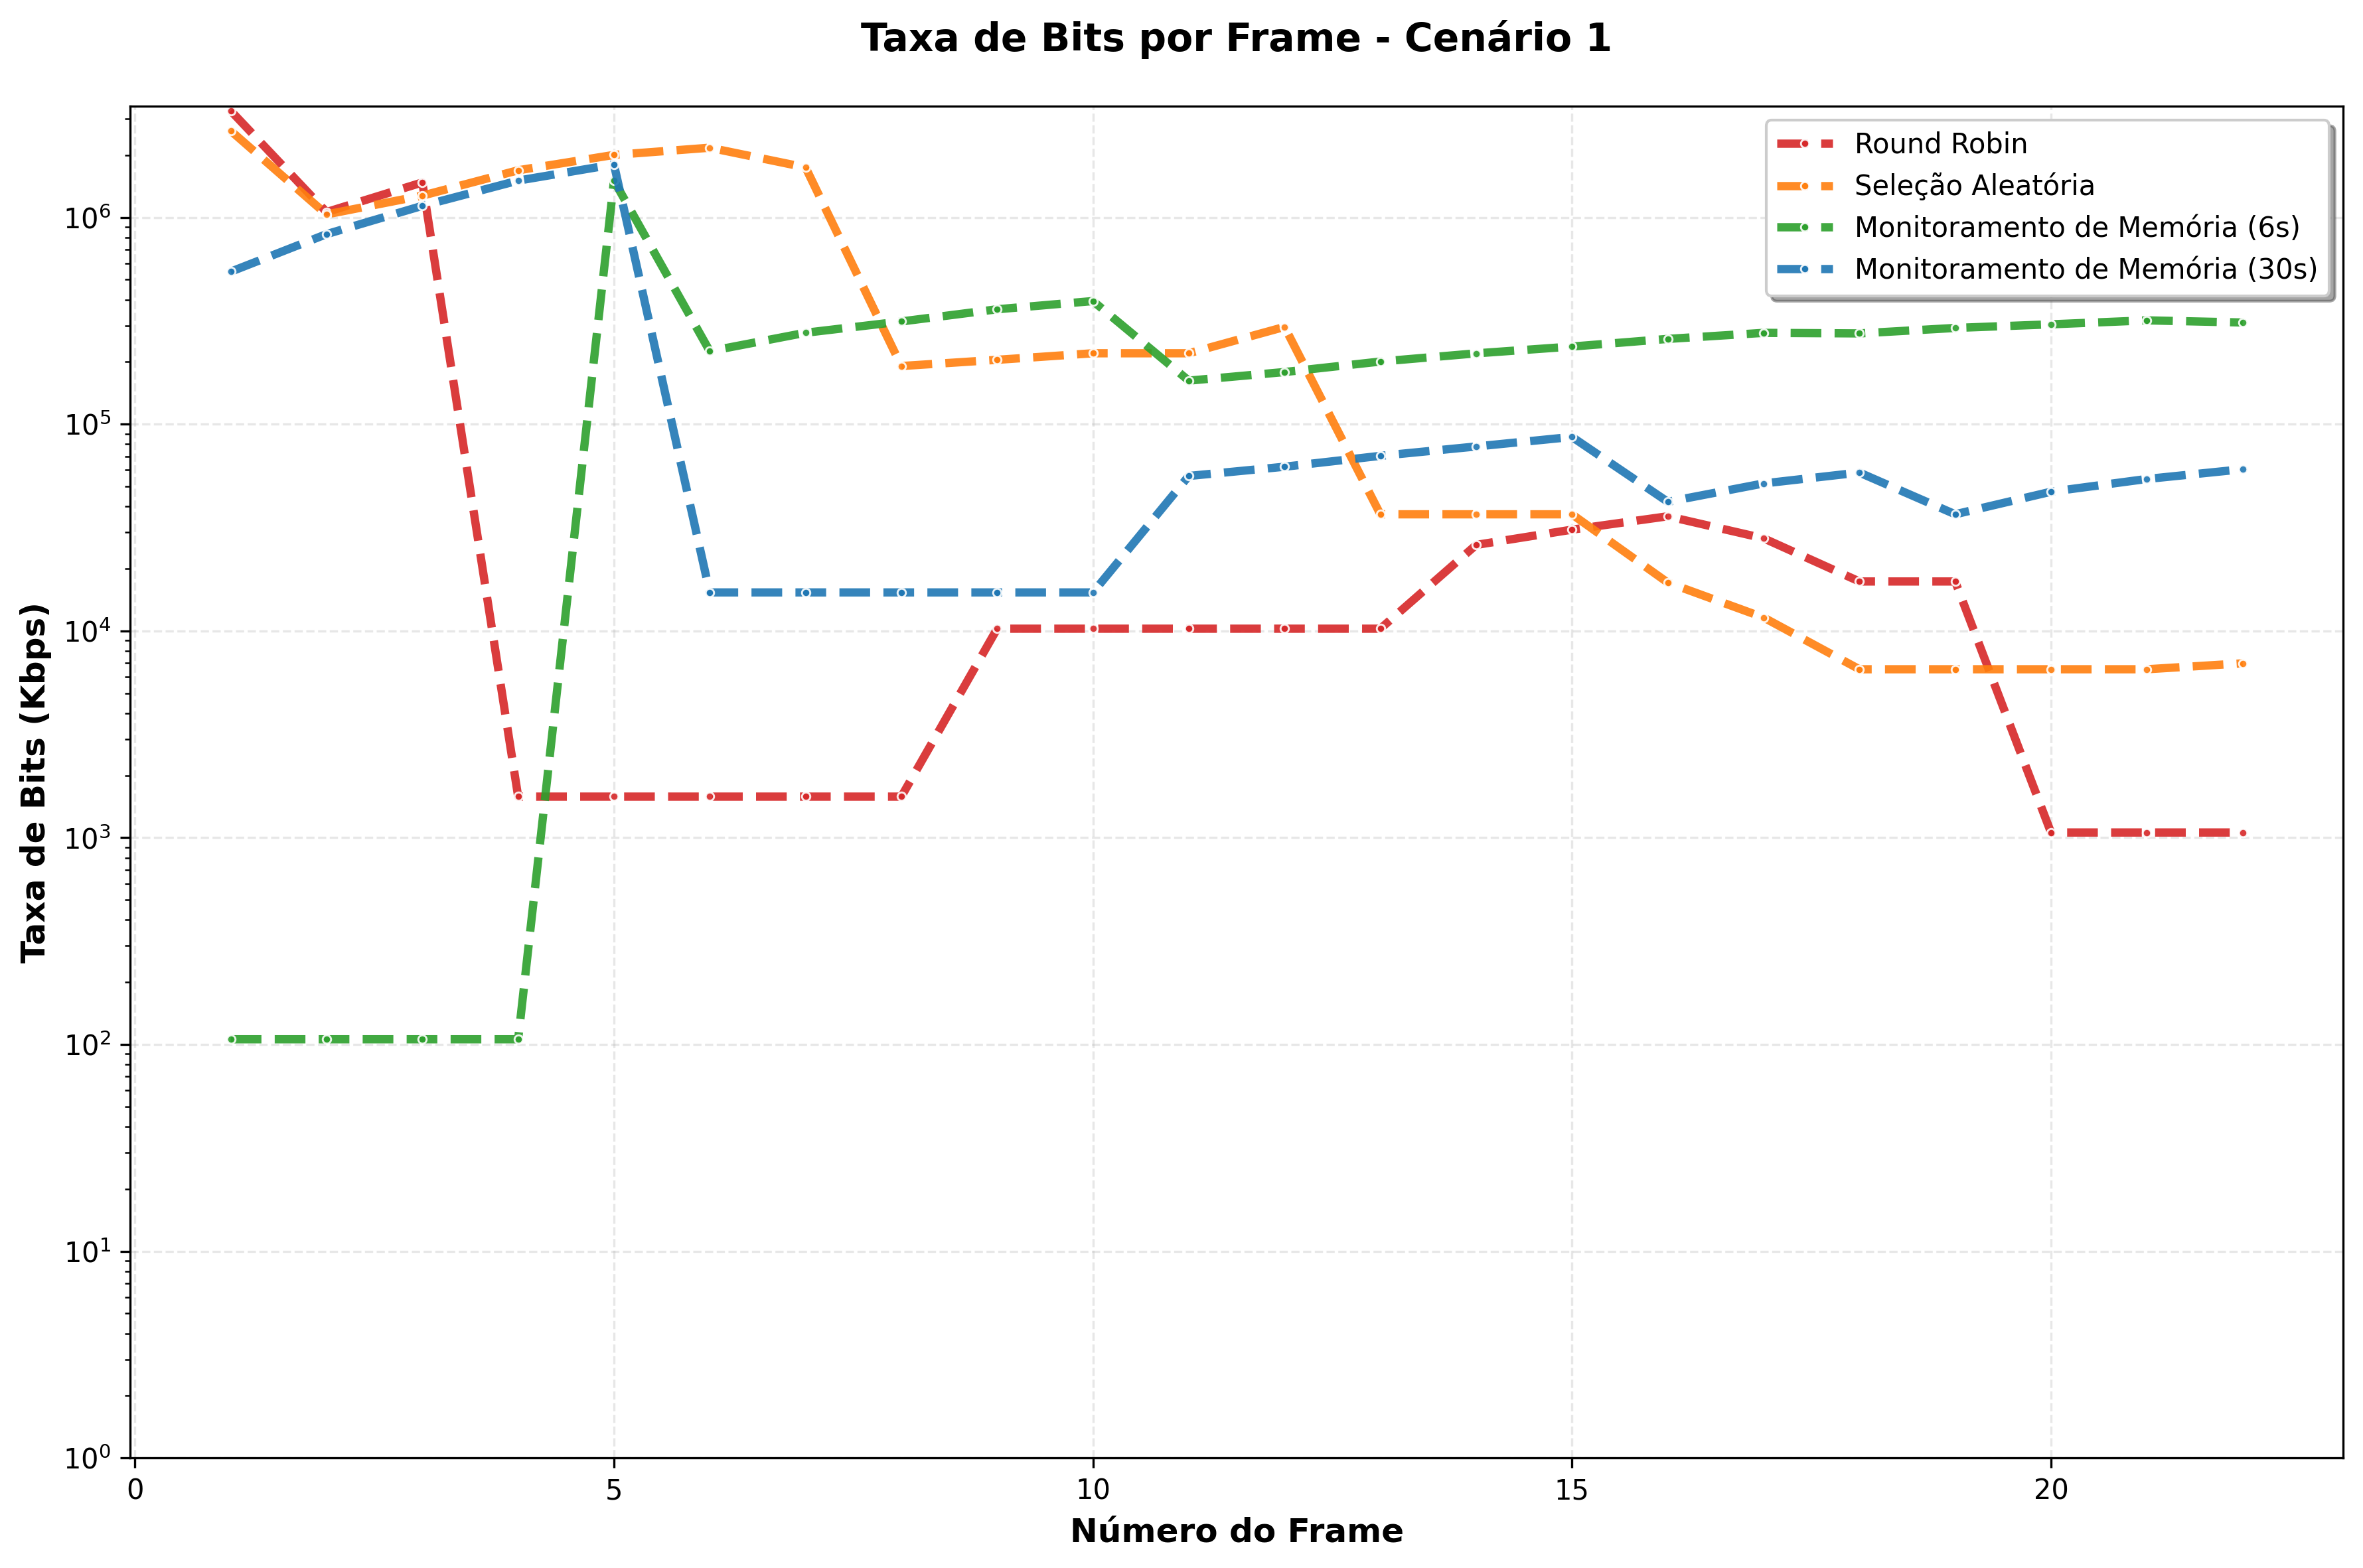
\includegraphics[width=0.75\linewidth]{./Textuais/5-ExperimentosEResultados/outputs/bitrate-charts/scenario-1.png}
    \caption{Evolução do \textit{bitrate} por segmento no Cenário 1 (100 usuários, servidores heterogêneos).}
    \text{Fonte: Elaborado pelo autor (2025).}
    \label{fig:bitrate-scenario-1}
\end{figure}

\begin{figure}[htbp]
    \centering
    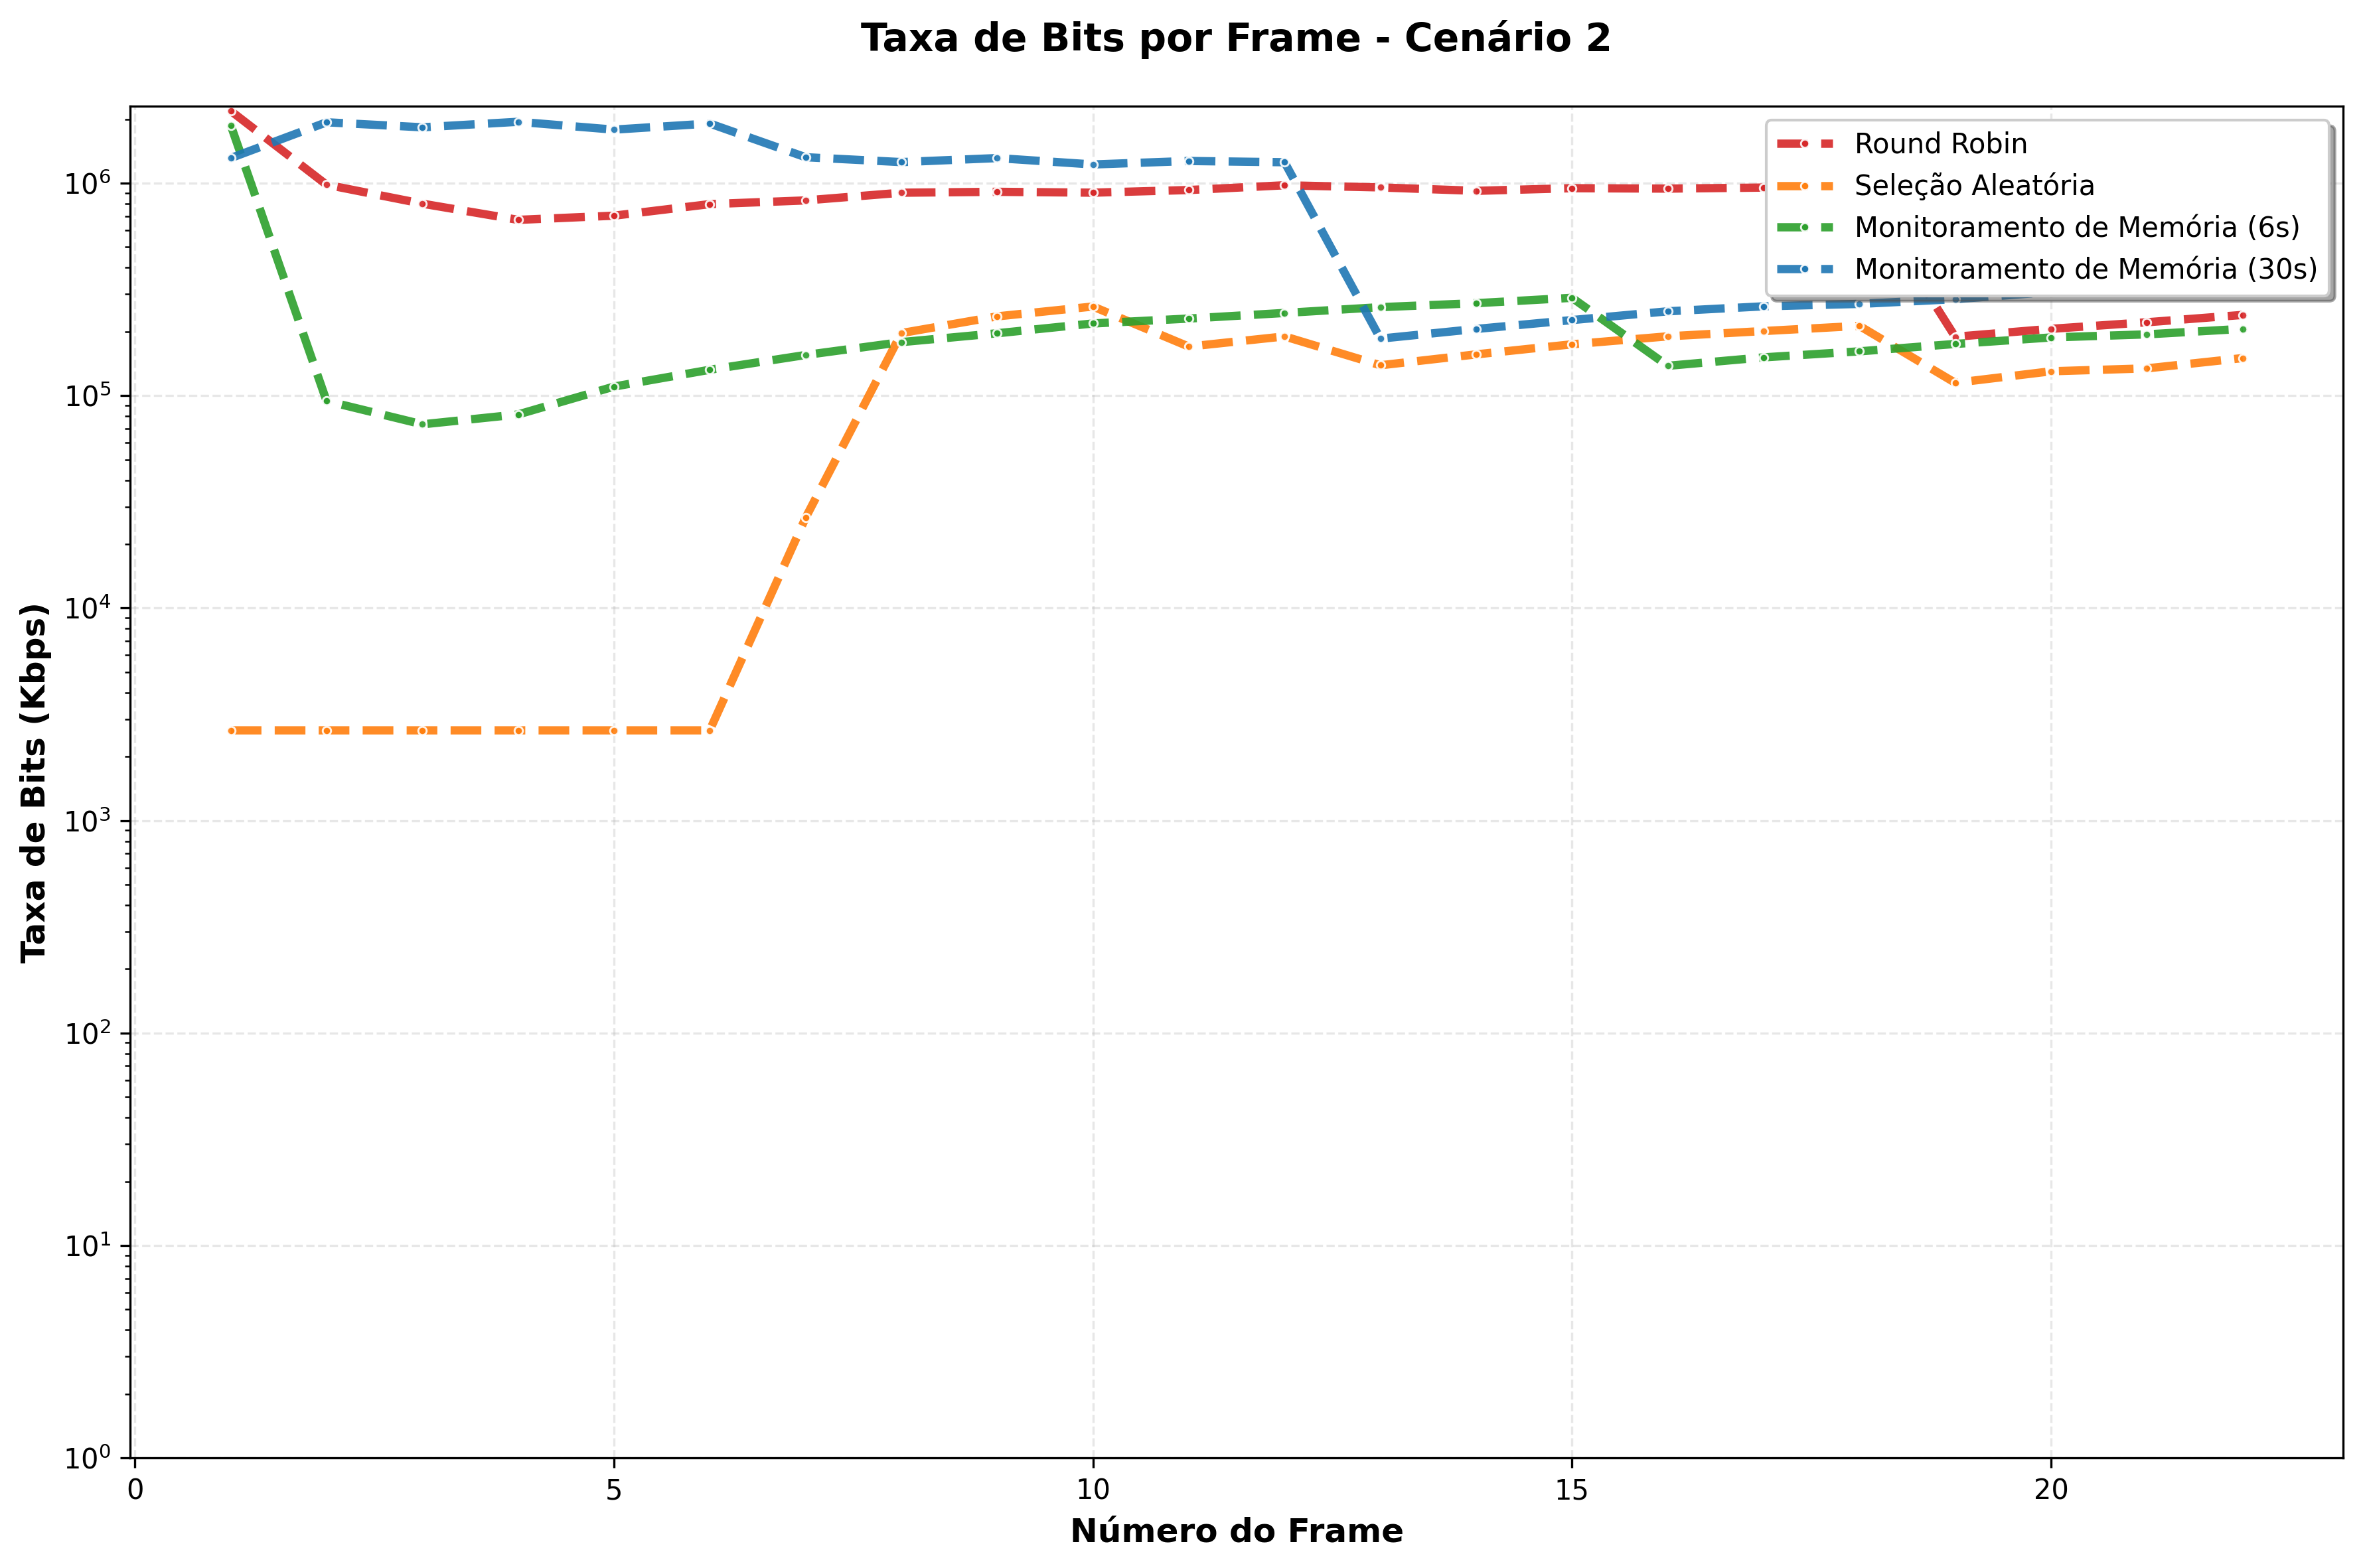
\includegraphics[width=0.75\linewidth]{./Textuais/5-ExperimentosEResultados/outputs/bitrate-charts/scenario-2.png}
    \caption{Evolução do \textit{bitrate} por segmento no Cenário 2 (100 usuários, servidores homogêneos).}
    \text{Fonte: Elaborado pelo autor (2025).}
    \label{fig:bitrate-scenario-2}
\end{figure}

\begin{figure}[htbp]
    \centering
    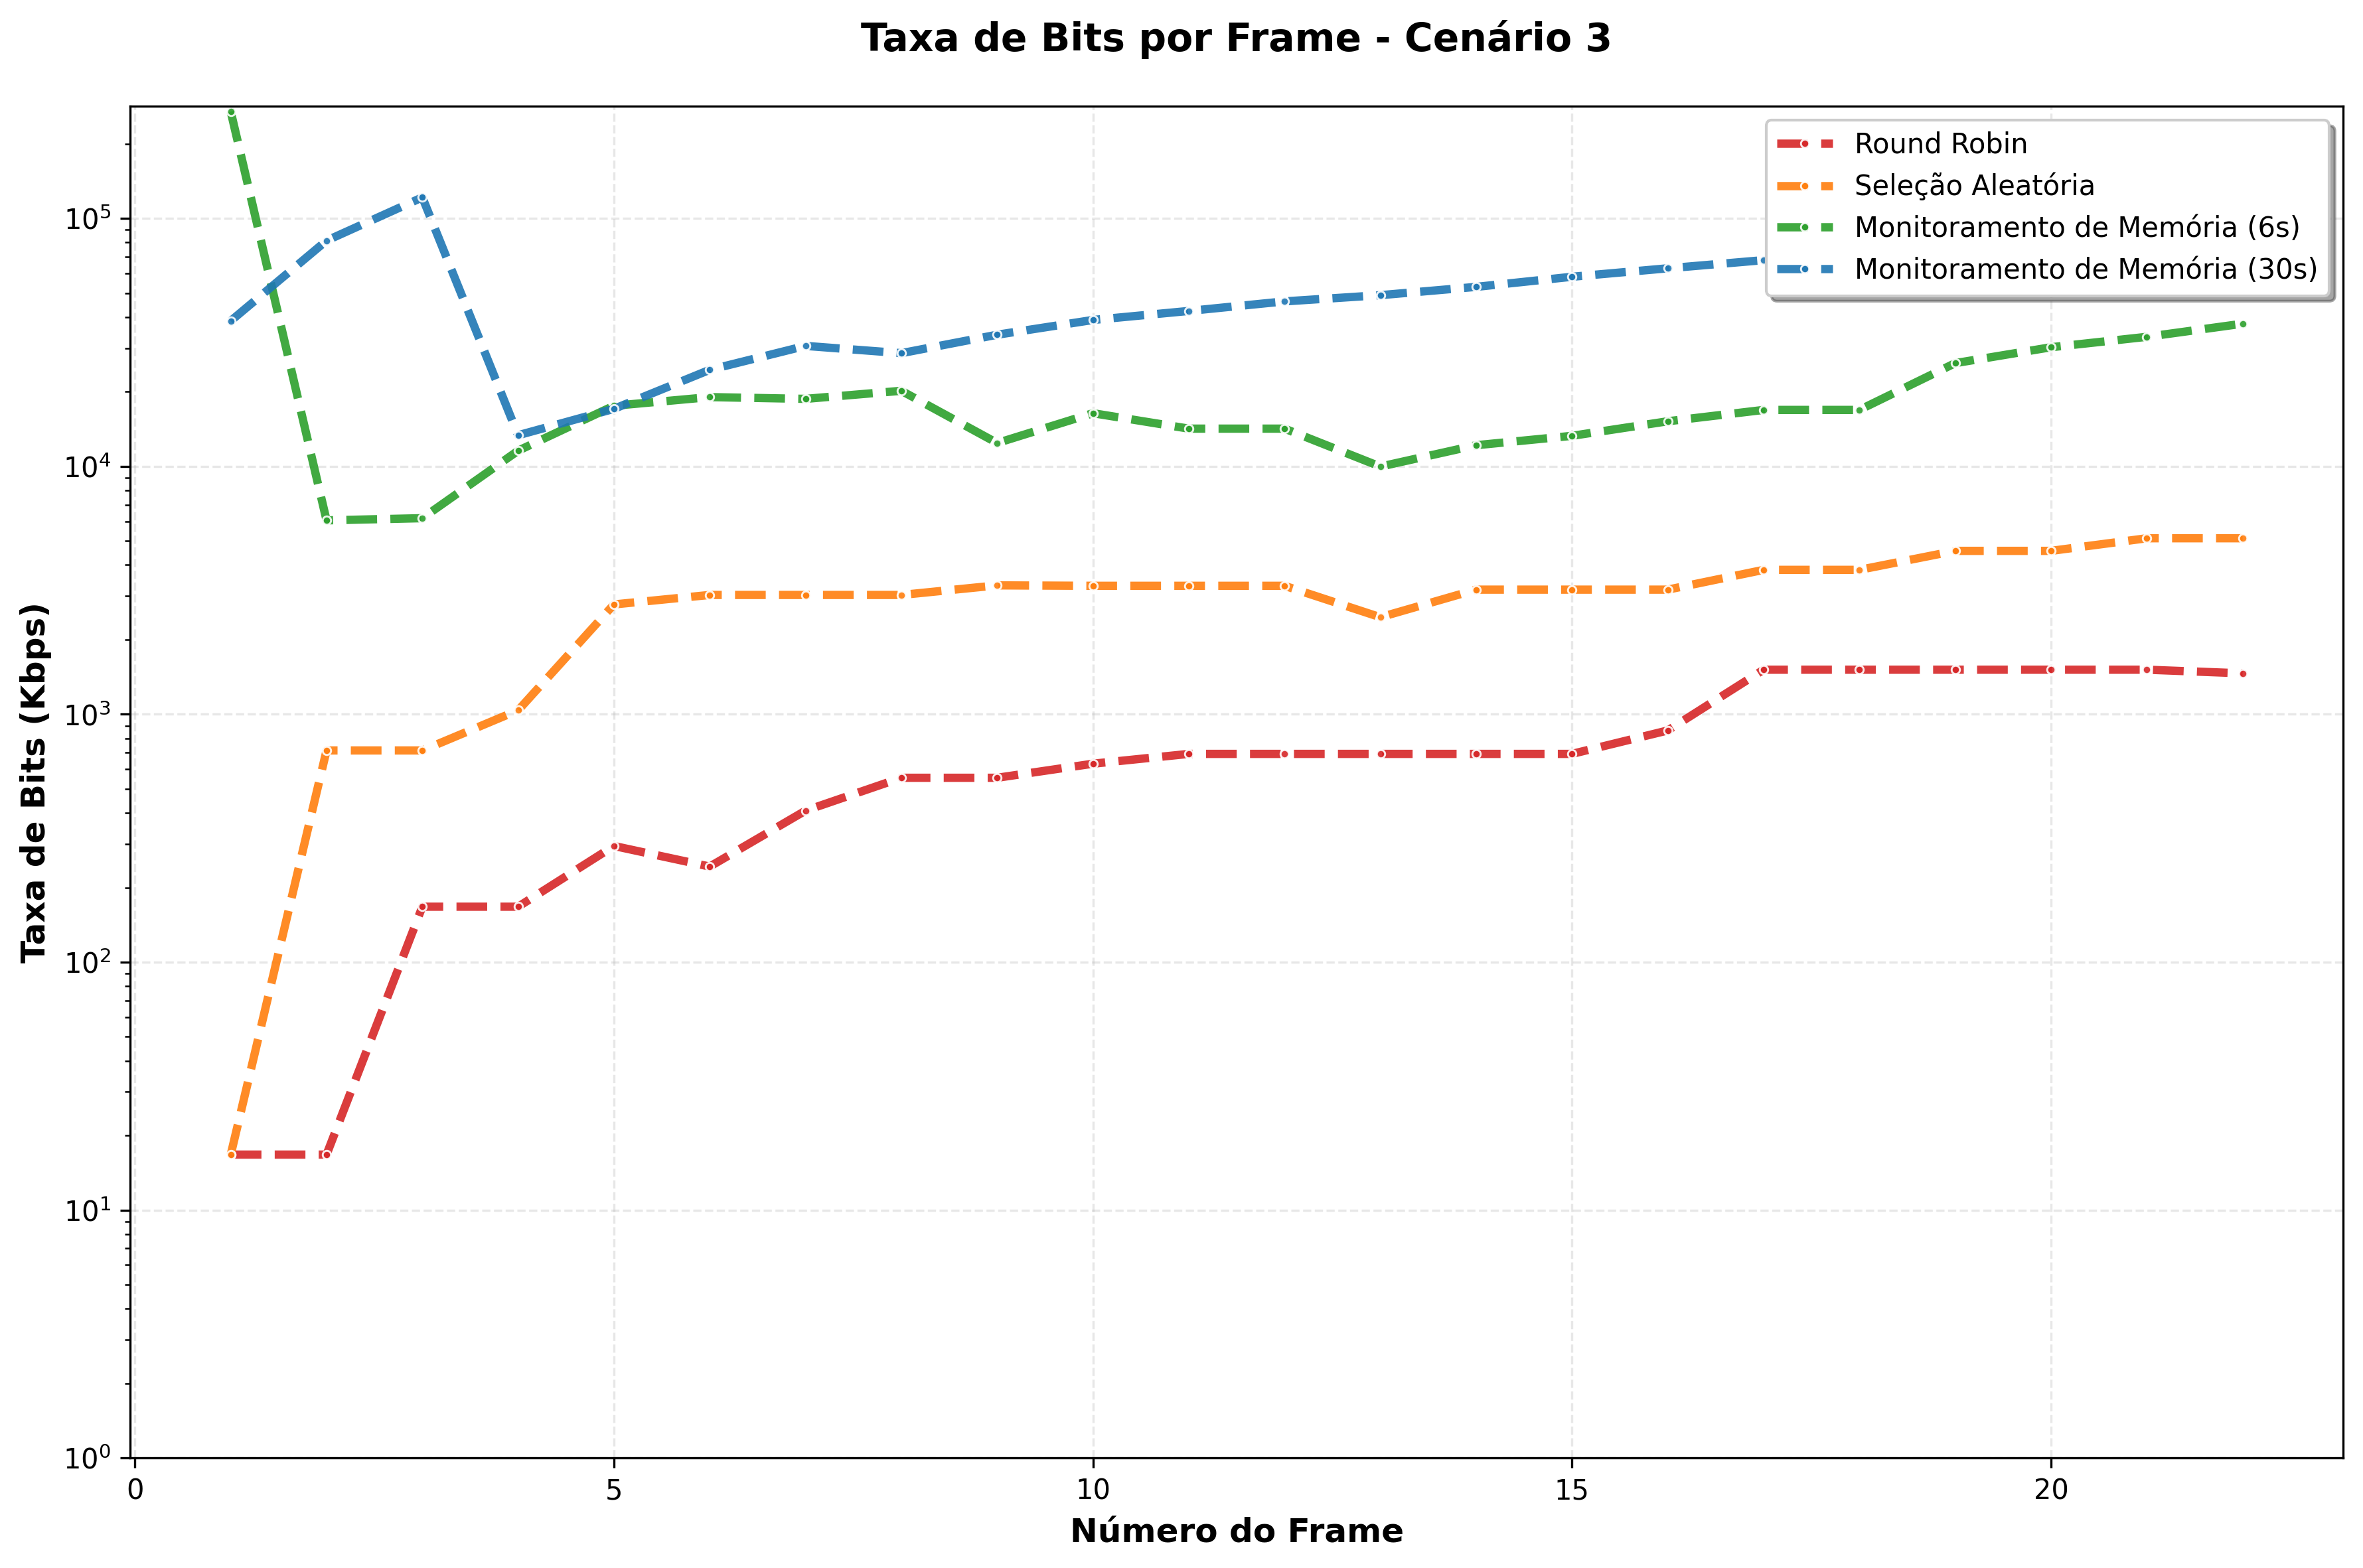
\includegraphics[width=0.75\linewidth]{./Textuais/5-ExperimentosEResultados/outputs/bitrate-charts/scenario-3.png}
    \caption{Evolução do \textit{bitrate} por segmento no Cenário 3 (1000 usuários, servidores heterogêneos).}
    \text{Fonte: Elaborado pelo autor (2025).}
    \label{fig:bitrate-scenario-3}
\end{figure}

\begin{figure}[htbp]
    \centering
    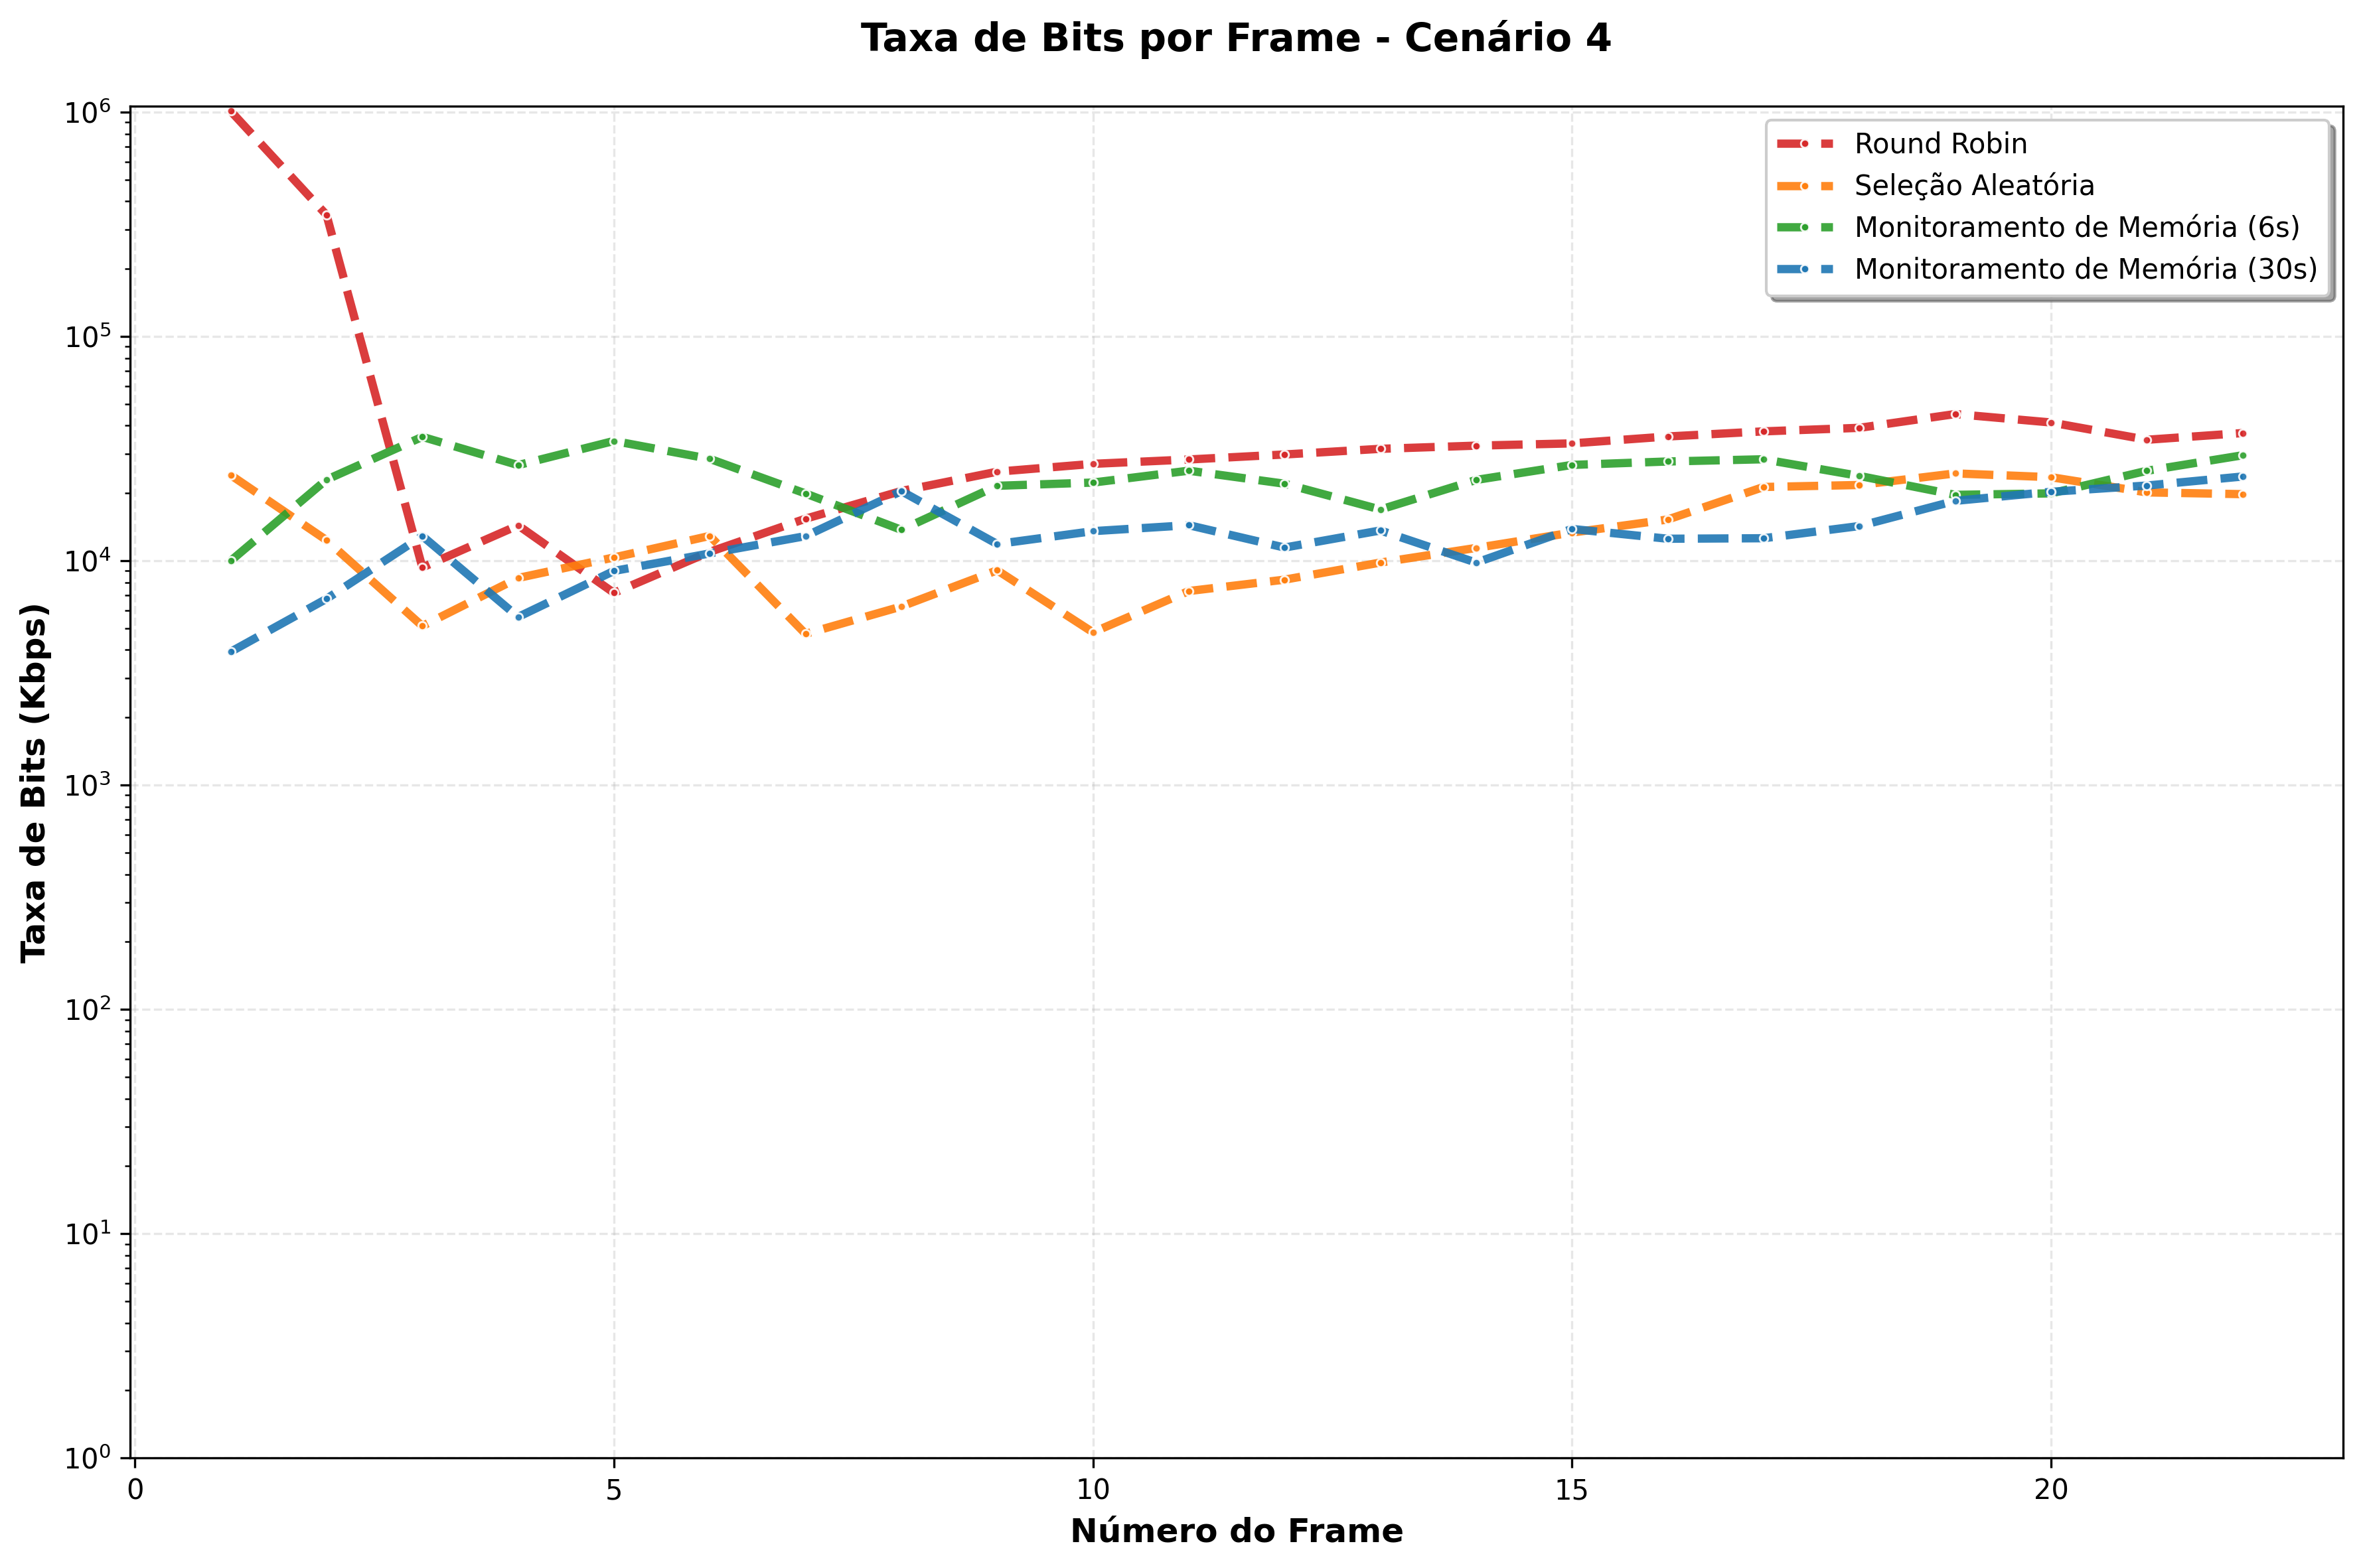
\includegraphics[width=0.75\linewidth]{./Textuais/5-ExperimentosEResultados/outputs/bitrate-charts/scenario-4.png}
    \caption{Evolução do \textit{bitrate} por segmento no Cenário 4 (1000 usuários, servidores homogêneos).}
    \text{Fonte: Elaborado pelo autor (2025).}
    \label{fig:bitrate-scenario-4}
\end{figure}

Nos cenários heterogêneos, o \textit{bitrate} alcançado pelas estratégias \textit{Round-Robin} e Seleção Aleatória apresenta picos isolados seguidos de quedas acentuadas e prolongadas, coerentes com as oscilações de qualidade observadas anteriormente. Em diversos instantes, os valores de \textit{bitrate} caem para patamares muito baixos, sinalizando que os clientes estão recebendo dados em ritmo insuficiente para sustentar resoluções altas sem comprometer a experiência de reprodução.

Já o algoritmo baseado em Monitoramento de Memória produz curvas de \textit{bitrate} mais estáveis, com valores consistentemente elevados ao longo dos segmentos. No Cenário 3, por exemplo, os dados JSON mostram que as variantes de Monitoramento de Memória mantêm \textit{bitrates} altos mesmo em momentos em que as estratégias tradicionais apresentam forte degradação. Isso reforça a hipótese de que considerar a carga real (memória e disco) permite explorar melhor a capacidade dos servidores mais robustos, evitando gargalos nos nós mais frágeis.

Nos cenários homogêneos, todas as estratégias apresentam \textit{bitrate} elevado e relativamente estável, com diferenças pequenas entre si. Tal como na análise de qualidade, isso indica que, quando os servidores possuem capacidades equivalentes, o simples balanceamento uniforme de requisições é suficiente para utilizar adequadamente os recursos disponíveis.

\subsection{Número de \textit{stalls}}

Além do resumo de travamentos apresentado na Tabela~\ref{tab:stalls-results}, foram gerados gráficos que mostram a distribuição dos eventos de \textit{stall} por segmento e por estratégia, permitindo visualizar em que momentos da sessão ocorrem as interrupções e qual sua duração relativa. As Figuras~\ref{fig:stall-scenario-1} a~\ref{fig:stall-scenario-4} apresentam essa distribuição para os quatro cenários investigados.

\begin{figure}[htbp]
    \centering
    
\includegraphics[width=0.75\linewidth]{./Textuais/5-ExperimentosEResultados/outputs/stall-charts/scenario-1.png}
    \caption{Distribuição dos eventos de \textit{stall} no Cenário 1 (100 usuários, servidores heterogêneos).}
    \text{Fonte: Elaborado pelo autor (2025).}
    \label{fig:stall-scenario-1}
\end{figure}

\begin{figure}[htbp]
    \centering
    
\includegraphics[width=0.75\linewidth]{./Textuais/5-ExperimentosEResultados/outputs/stall-charts/scenario-2.png}
    \caption{Distribuição dos eventos de \textit{stall} no Cenário 2 (100 usuários, servidores homogêneos).}
    \text{Fonte: Elaborado pelo autor (2025).}
    \label{fig:stall-scenario-2}
\end{figure}

\begin{figure}[htbp]
    \centering
    
\includegraphics[width=0.75\linewidth]{./Textuais/5-ExperimentosEResultados/outputs/stall-charts/scenario-3.png}
    \caption{Distribuição dos eventos de \textit{stall} no Cenário 3 (1000 usuários, servidores heterogêneos).}
    \text{Fonte: Elaborado pelo autor (2025).}
    \label{fig:stall-scenario-3}
\end{figure}

\begin{figure}[htbp]
    \centering
    
\includegraphics[width=0.75\linewidth]{./Textuais/5-ExperimentosEResultados/outputs/stall-charts/scenario-4.png}
    \caption{Distribuição dos eventos de \textit{stall} no Cenário 4 (1000 usuários, servidores homogêneos).}
    \text{Fonte: Elaborado pelo autor (2025).}
    \label{fig:stall-scenario-4}
\end{figure}

Os dados mostram que, nos cenários heterogêneos, os \textit{stalls} associados às estratégias \textit{Round-Robin} e Seleção Aleatória concentram-se em segmentos específicos, frequentemente com durações significativas (como os trechos de 8{,}16s e 13{,}38s observados no Cenário 3). Esses eventos longos tendem a ocorrer em momentos em que múltiplos clientes competem por servidores limitados, refletindo a incapacidade das estratégias tradicionais de evitar sobrecarga em nós com menos recursos disponíveis.

Por outro lado, a variante de Monitoramento de Memória com intervalo de 6 segundos não registrou nenhum \textit{stall} nos cenários críticos, e a variante com 30 segundos apresentou poucos eventos, todos de curta duração, conforme já resumido na Tabela~\ref{tab:stalls-results}. Em cenários homogêneos (Cenários 2 e 4), os gráficos confirmam a inexistência de travamentos para todas as estratégias, reforçando a conclusão de que a heterogeneidade de recursos é o principal fator desencadeador de problemas severos de QoE.

\subsection{Latência}

Por fim, a latência média de resposta foi consolidada tanto na Tabela~\ref{tab:latency-results} quanto em um gráfico comparativo geral, apresentado na Figura~\ref{fig:latency-chart}. Essa métrica sintetiza o tempo médio necessário para completar cada requisição HTTP ao longo da sessão, agregando em um único valor o efeito combinado de processamento no balanceador, capacidade dos servidores e competição por recursos.

\begin{figure}[htbp]
    \centering
    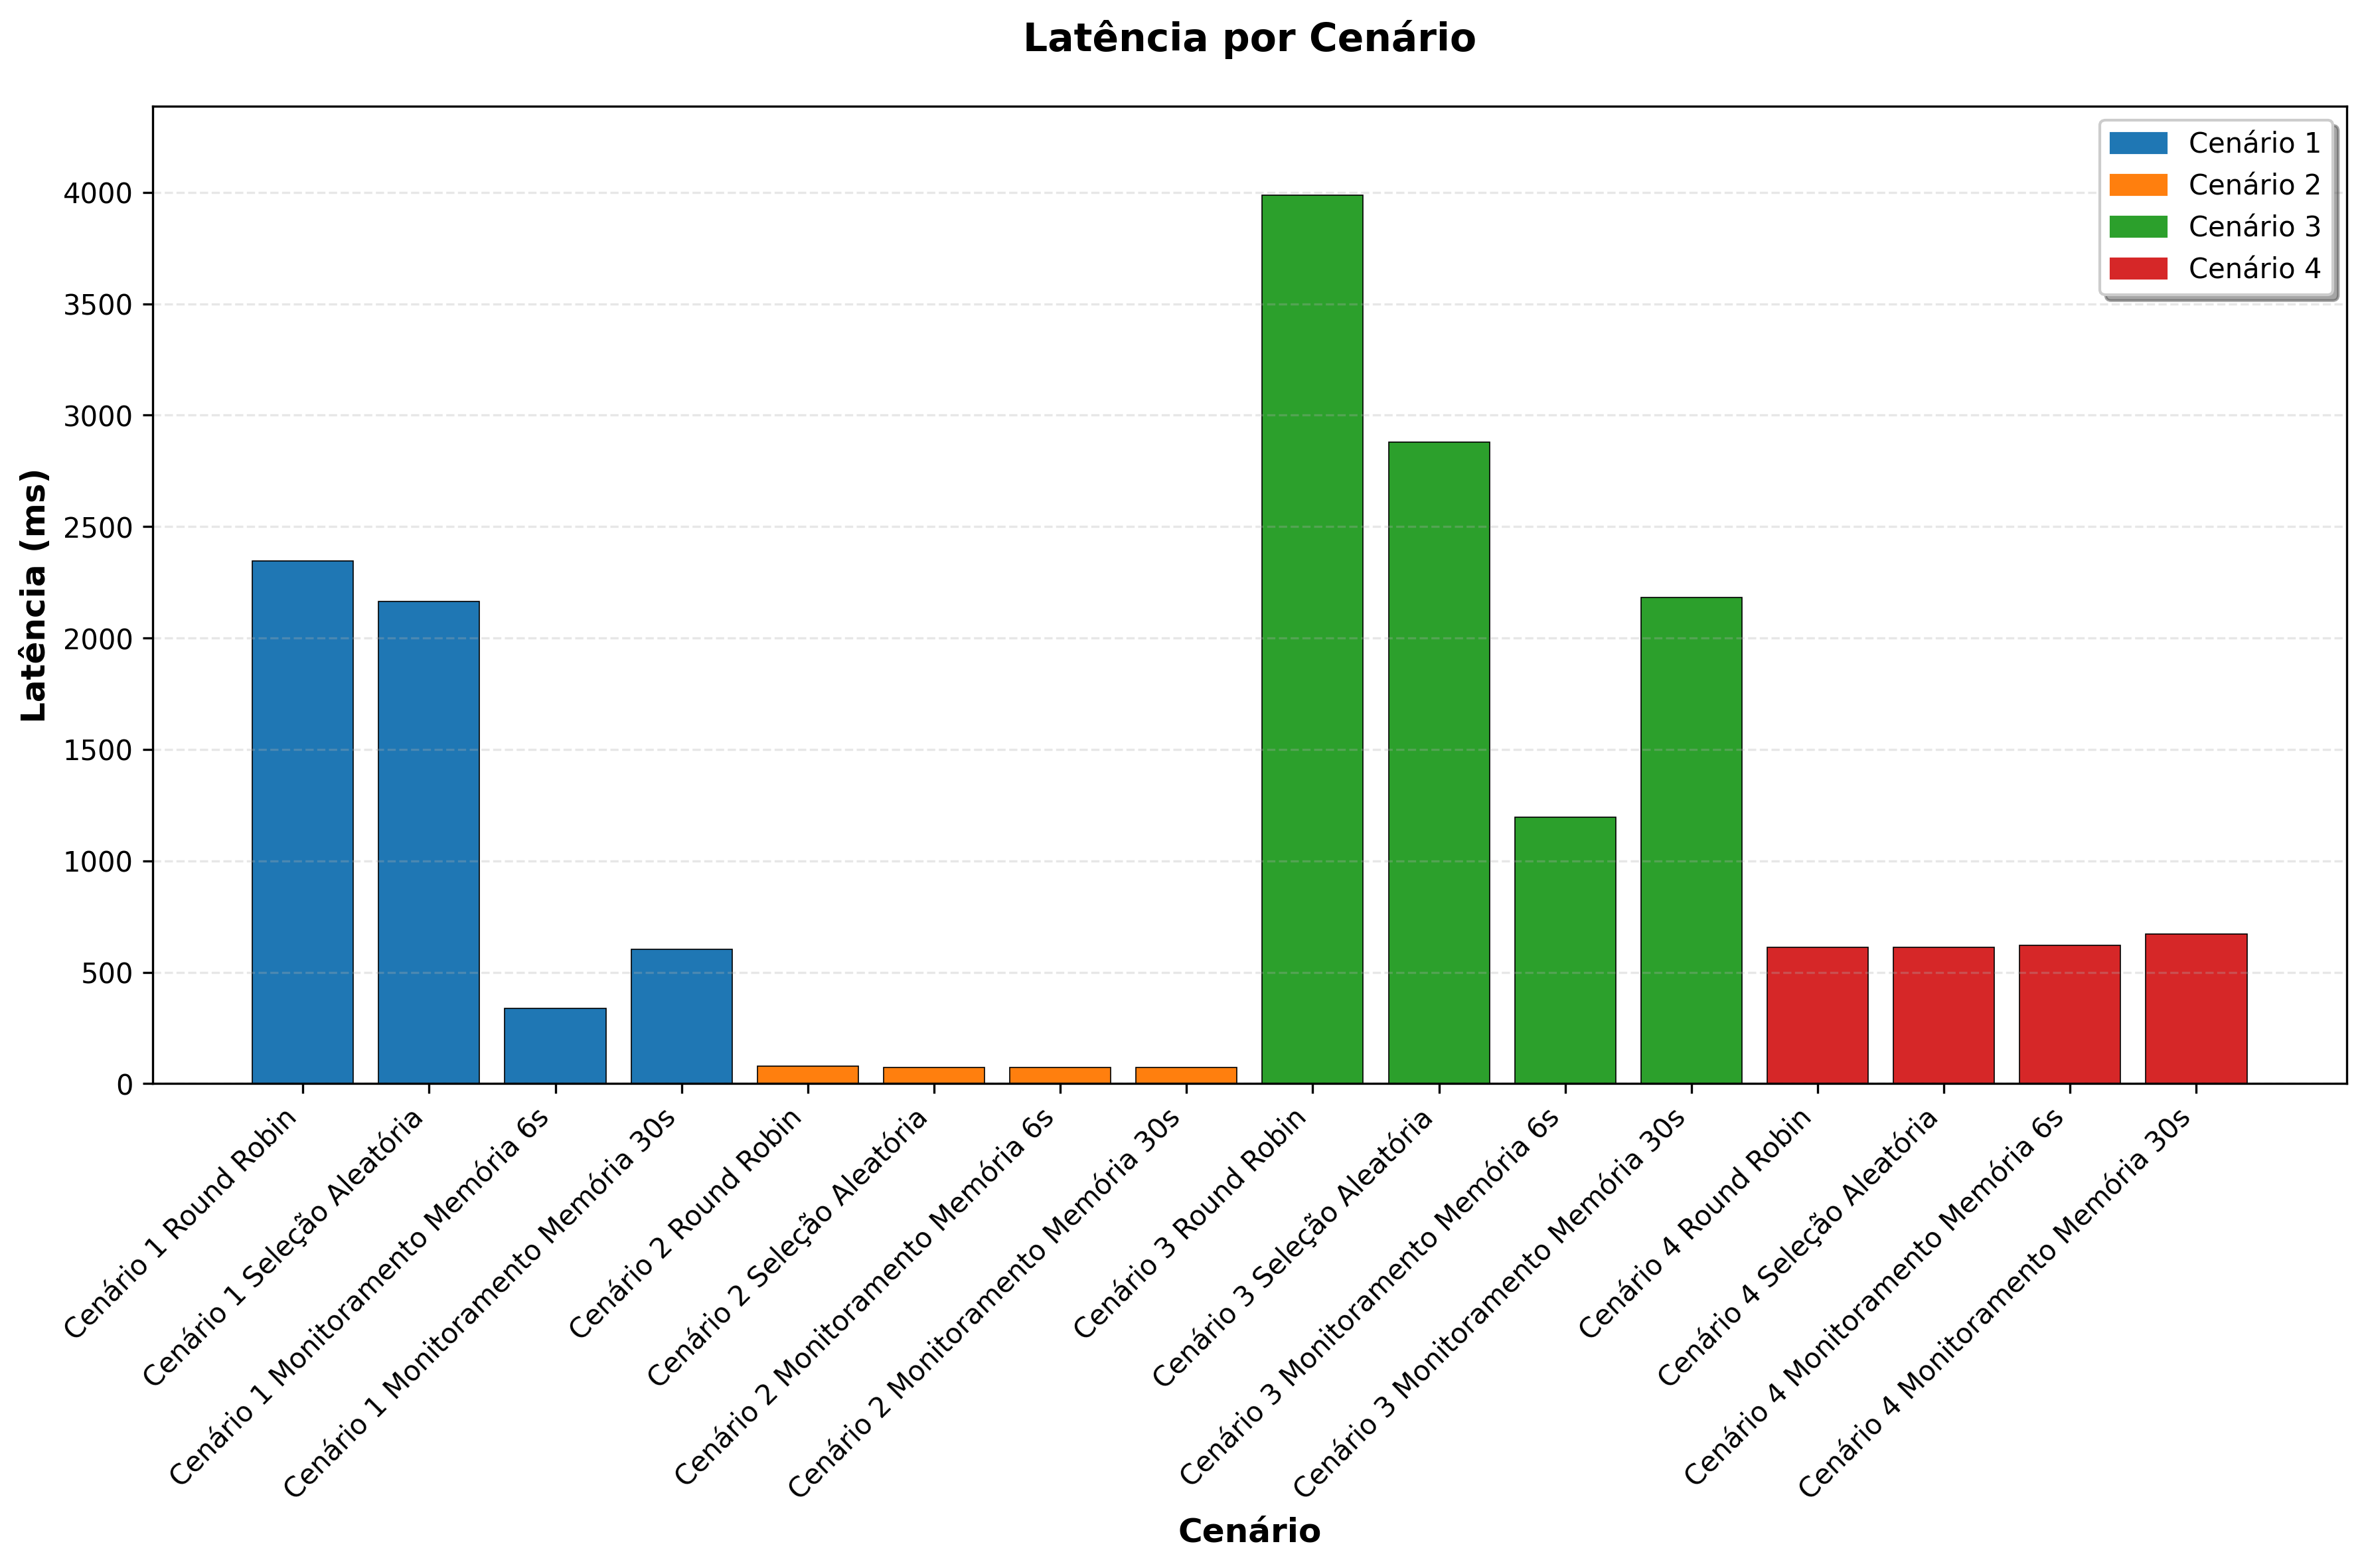
\includegraphics[width=0.85\linewidth]{./Textuais/5-ExperimentosEResultados/outputs/latency_chart.png}
    \caption{Comparação da latência média de resposta por cenário e estratégia de balanceamento.}
    \text{Fonte: Elaborado pelo autor (2025).}
    \label{fig:latency-chart}
\end{figure}

O gráfico deixa evidente que as maiores diferenças ocorrem em ambientes heterogêneos. No Cenário 1, o Monitoramento de Memória com intervalo de 6 segundos reduz a latência média de aproximadamente 2{,}3 segundos (\textit{Round-Robin}) para cerca de 0{,}33 segundos, enquanto no Cenário 3 a redução é de quase 4 segundos para pouco menos de 1{,}2 segundos. A variante com intervalo de 30 segundos, embora apresente latências um pouco maiores que a de 6 segundos, ainda se mantém muito abaixo das estratégias tradicionais, demonstrando boa robustez mesmo com informação moderadamente obsoleta.

Nos cenários homogêneos, as latências de todas as estratégias são bastante próximas, com valores sempre inferiores a 700 milissegundos. Isso indica que, quando os servidores possuem capacidades equivalentes, o impacto da estratégia de balanceamento na latência é relativamente pequeno, e que o overhead introduzido pelo monitoramento de memória e pela lógica probabilística do algoritmo proposto não compromete o tempo de resposta.

\section{Análise}

\subsection{Comparação entre heterogeneidade e homogeneidade}

Os resultados obtidos revelam claramente que o impacto do algoritmo proposto é muito mais expressivo em cenários com servidores heterogêneos. Nos Cenários 1 e 3, as métricas de qualidade, \textit{bitrate}, \textit{stalls} e latência convergem para uma mesma conclusão: estratégias que ignoram o estado dos servidores tendem a sobrecarregar nós com menos recursos disponíveis, produzindo quedas severas de qualidade, aumento de travamentos e latências elevadas. Em contrapartida, o Monitoramento de Memória utiliza as métricas de uso de RAM e leitura de disco para concentrar o tráfego em servidores mais capazes, mitigando esses efeitos adversos.

Nos cenários homogêneos (Cenários 2 e 4), por outro lado, as diferenças entre as estratégias tornam-se discretas. Todos os algoritmos conseguem manter alta qualidade, inexistência de travamentos e latências reduzidas, uma vez que não há servidores com menos recursos disponíveis a serem evitados. Isso sugere que o principal benefício da abordagem proposta está na capacidade de explorar de forma inteligente a heterogeneidade de recursos, cenário comum em CDNs reais, nas quais servidores com perfis distintos coexistem em uma mesma infraestrutura.

\subsection{Impacto do intervalo de atualização}

O intervalo de atualização das métricas representa diretamente o grau de obsolescência da informação de carga utilizada pelo algoritmo de balanceamento. Os experimentos com 6 e 30 segundos demonstram que, embora a informação mais recente (6s) produza os melhores resultados absolutos em termos de latência e travamentos, o algoritmo mantém desempenho significativamente superior às estratégias tradicionais mesmo com dados mais antigos (30s).

No Cenário 3, por exemplo, ambas as variantes de Monitoramento de Memória preservam a qualidade em resoluções altas e eliminam ou reduzem drasticamente os \textit{stalls}, mas a configuração de 6 segundos é a única que zera completamente os travamentos e apresenta a menor latência média. Já a variante de 30 segundos, embora apresente alguns \textit{stalls} curtos e latência um pouco maior, ainda se distancia amplamente de \textit{Round-Robin} e Seleção Aleatória. Esses resultados são coerentes com a fundamentação teórica discutida no Capítulo~\ref{cap:Proposta}: a interpretação adequada de dados obsoletos permite amortecer o impacto da defasagem temporal, mas intervalos menores de atualização potencializam o aproveitamento das informações mais recentes.

\subsection{Análise da QoE de modo geral}

Sob a perspectiva da experiência do usuário final, o conjunto de métricas analisadas converge para um quadro consistente. Em cenários homogêneos, todas as estratégias fornecem uma QoE elevada, com reprodução contínua em alta definição, ausência de travamentos e tempos de resposta satisfatórios. Nesses casos, o algoritmo proposto mantém desempenho comparável às estratégias tradicionais, demonstrando que o custo adicional de monitoramento e cálculo probabilístico não introduz penalidades perceptíveis.

Em cenários heterogêneos, entretanto, as diferenças são decisivas. A combinação de latências elevadas, múltiplos \textit{stalls} longos e degradação para resoluções muito baixas observada em \textit{Round-Robin} e Seleção Aleatória (especialmente no Cenário 3) representa uma deterioração significativa da QoE. O algoritmo de Monitoramento de Memória, por sua vez, praticamente elimina os travamentos, reduz substancialmente a latência e mantém a maior parte da sessão em 720p ou 1080p, mesmo sob alta concorrência. Assim, os resultados experimentais confirmam a hipótese central do trabalho: o uso de métricas de memória e disco, interpretadas à luz da obsolescência da informação de carga, é eficaz para melhorar a qualidade de experiência em sistemas de distribuição de conteúdo sujeitos a cenários de carga desafiadores.
